\documentclass{article}
\usepackage[legalpaper, portrait, margin=1in]{geometry}
\usepackage{graphicx}

\title{CS422 Project 4 PCA}
\author{Nicholas Ang}
\date{December 2022}

\begin{document}

\maketitle
\clearpage
\section*{Principal Component Analysis}
\subsection*{Implementation}
In my implementation, I did not standardize or center my data. I calculated the covariance matrix, principal components, and data projection using the given Z matrix. The covariance matrix is calculated using matrix multiplication between Z transpose and Z. The principal components are calculated by finding the eigenvalues and eigenvectors of the covariance matrix. The projected data is calculated by matrix multiplying Z and the most important principal component. The original data is plotted in blue while the projected data is plotted in orange. 
\begin{figure}[!htb]
    \centering
    \textbf{PCA Plotting with Test Data 1}\par
    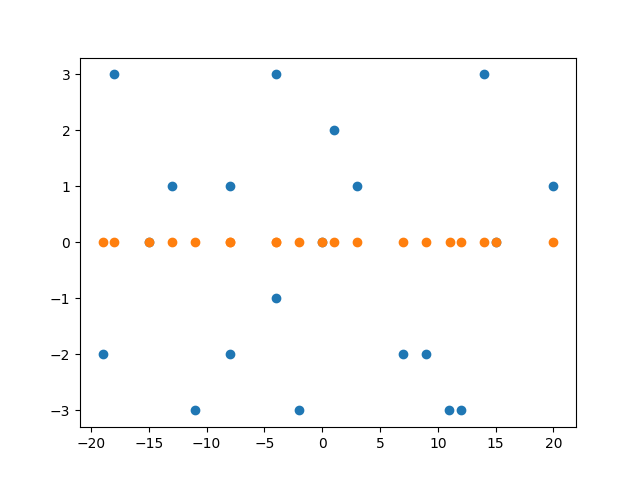
\includegraphics[width=14cm]{Images/test_data_1_plot.jpg}
    \newline
    \textbf{PCA Plotting with Test Data 2}\par
    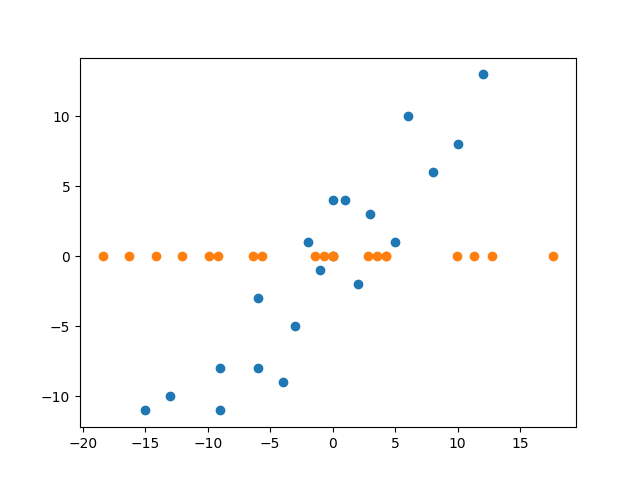
\includegraphics[width=14cm]{Images/test_data_2_plot.jpg}
\end{figure}
\subsection*{Benefits with Higher Dimensional Feature Vectors}
Principal component analysis is very useful in simplifying the data while retaining the most important information. With PCA, it selects which features cause the most variance and have the most important features. With a lot of dimensions, it focuses on what mostly causes the changes in the data. For example, if there are three features and two features account for ninety five percent of the variance, the third feature does not offer much information and PCA can be used to reduce the dimensions to the two features that provide the most information. It essentially removes features that do not majorly impact the data. Another benefit is that since PCA reduces dimensions, it makes it easier to apply different machine learning techniques and visualize the data. For example, I could use PCA to reduce the features of a data set to two features and then graph the data. The data can then be clustered using something like K-means and analyzed in a easier way.
\end{document}
